\documentclass{article}

\usepackage{amsmath}
\usepackage{amssymb}
\usepackage{graphicx}
% \usepackage[usenames]{color}
% \definecolor{gray}{RGB}{128,128,128}
%\usepackage[bookmarks={false},%
%pdftex,%
%unicode,%
%colorlinks,%
%citecolor={gray},%
%filecolor={gray},%
%linkcolor={gray},%
%urlcolor={gray},%
%pdfauthor={Bob Carpenter},%
%pdftitle={A Hierarchical Bayesian Model of Crowdsourced Relevance Coding}%
%]%
%{hyperref}

\setlength{\textheight}{9.0in}
\setlength{\textwidth}{6.5in}
\setlength{\oddsidemargin}{0.0in}
\setlength{\topmargin}{-0.5in}

\renewcommand{\floatpagefraction}{0.95}
\title{A Hierarchical Bayesian Model of\\ 
Crowdsourced Relevance Coding}
\author{Bob Carpenter
\\[4pt] Columbia University, Department of Statistics
\\[4pt] LingPipe, Inc.
\\[4pt] \texttt{carp@lingpipe.com}}

\begin{document}

\maketitle

\abstract{We apply a generative probabilistic model of noisy
crowdsourced coding to overlapping relevance judgments for documents
in several topics (queries).  We demonstrate the model's utility for
Task 2 of the 2011 TREC Crowdsourcing Track (Karzai and Lease 2011).

Our model extends Dawid and Skene's (1979) approach to inferring gold
standards from noisy coding in several ways: we add a hierarchical
model of prevalence of relevant documents in multiple topics
(queries), semi-supervision using known gold labels, and
hierarchically modeled priors for coder sensitivity and specificity.
We also replace Dawid and Skene's maximum likelihood point estimates
with full Bayesian inference using Gibbs sampling and generalize
their full-panel design in which every coder labels every document
to a fully ad hoc design in which a coder may label each document
zero, one or more times.}


\section{The Data}

The training data consists of overlapping crowdsourced relevance
judgments for pairs of queries and documents along with a seed set of
known gold-standard labels.  The underlying data was
collected by Wei and Lease (2011) using Amazon's Mechanical Turk 
with gold-standard labels provided by NIST.  The data that was
annotated is a subset of document/topic pairs for which the documents
were judged relevant by systems in the the 2010 TREC Relevance
Feedback track. 

Although originally collected on a three-point scale (highly relevant,
relevant and irrelevant), the two relevant categories were collapsed
for this evaluation.

The data revolves around 100 different structured queries, which are
called ``topics'' in TREC evaluations.  The topics themselves are not
part of the data for the evaluation in the sense that the only
information we have about a topic is an identification number.

A total of 19,033 topic/document pairs were annotated by workers.  The
documents themselves are not part of the data for the evaluation, being
available only as identification numbers.

A total of 762 workers participated in coding the data, each
annotating differeing sized subset of the topic/document pairs.  Like
the topics and documents, the only information we have about the
workers is an identification number.

Gold-standard judgments (as labeled by NIST) are provided for a total of
2275 topic/document pairs.  An additional 1000 gold-standard judgments
on topic/document pairs were held out and will be used for evaluation.

An additional 16,758 topic/document pairs
are provided with no gold-standard judgment, bringing the total to
19,033 topic/document pairs. 

For the 2275 topic/document pairs with gold labels, there are an
additional 13,749 worker-supplied labels.  For the 16,758
topic/document pairs without gold-standard labels, there are
75,875 worker-supplied labels.


\section{The Evaluation}

There are two subtasks making up Task 2 of the TREC 2011 Crowdsourcing
Track.  

The first subtask is to provide categorical relevance judgments for
each topic/document pair (0 for irrelevant and 1 for relevant).
These judgments may be fractions between 0 and 1.

Evaluation for the first task is with the traditional IR measures of
precision (TP/[TP+FP]) and recall/sensitivity (TP/[TP+FN]).  Because
precision and recall ignore true negatives, we've been lobbying to
also have specificity (TN/[TN+FP]) evaluated.  

Given these measures, we are skeptical about the utility of fractional
judgments (see section~\ref{confusion-matrix-eval-sec}).  

The second subtask is to rank the documents by relevance for each
topic.  These will be scored by standard TREC ranking evaluations.


\section{Overview of Our Entries}

We have entered three systems based on a semi-supervised model and an
unsupervised model.  For two of these entries, we quantize results to
0 or 1.  For one entry, we use a Bayesian estimator of relevance
probability.  Specifically, we're minimizing expected squared
estimation error, which amounts to using posterior averages for
estimates.  This is {\it not}\ a method that's tuned to the
evaluation.

For all entries, we rank based on our Bayesian estimates of
relevance probability.  


\section{The Model}

\subsection{Constants}

Data sizes are given by the following unmodeled constants.
%
\begin{itemize}
\item $J > 0$: number of coders
\item $T > 0$: number of topics (i.e., queries)
\item $I > 0$: number of document/topic pairs
\item $K > 0$: number of judgments (i.e., labels)
\end{itemize}
%
In a complete panel design, every coder would judge each
document/topic pair exactly once.  Because of the mixed design of
the TREC data, it is convenient to use the following constant indexing arrays.
%
\begin{itemize}
\item $tt[i] \in 1{:}T$: topic for document/topic pair $i \in 1{:}I$
\item $jj[k] \in 1{:}J$: worker for judgment $k \in 1{:}K$
\item $ii[k] \in 1{:}I$: document/topic pair for judgment $k \in 1{:}K$
\end{itemize}

\subsection{Variables}

The lowest-level random variables in the model are discrete.
%
\begin{itemize}
\item $z[i] \in \{0, 1\}$: relevance of document/topic pair $i \in 1{:}I$
\item $y[k] \in \{0, 1\}$: label provided by worker $jj[k]$ for
document/topic pair $ii[k]$ for judgment $k \in 1{:}K$
\end{itemize}
%
The labels $y$ are fully observed.  In the unsupervised case the true
relevances $z_i$ are unknown.  In the semi-supervised case, values of
$z_i$ for are known for for some document/topic pairs $i$.

The labels and relevances are characterized by the following continuous parameters.
%
\begin{itemize}
\item $\pi[t] \in [0,1]$: prevalence of relevant documents in topic $t \in
1{:}T$
\item $\theta_0[j] \in [0,1]$: specificity of worker $j \in 1{:}J$
\item $\theta_1[j] \in [0,1]$: sensitivity of worker $j \in 1{:}J$
\end{itemize}
%
The continuous parameters have priors, which characterize their distributions.
%
\begin{itemize}
\item $\phi_{\pi}, \phi_0, \phi_1  \in (0,1)$: prior mean for
prevalence, specificity, and sensitivity
\item $\kappa_{\pi}, \kappa_0, \kappa_1 \in (0,\infty)$: prior count
size for prevalence, specificity, and sensitivity
\end{itemize}
%
In our Bayesian hierarchical model, we also treat these as variable
and provide one additional level of hard coded priors for them.  The
sensitivity and specificity parameters characterize the population of
coders in terms of average accuracy, average bias, and the
variation among coder accuracies and biases.  For the prevalence parameters,
these priors characterize the mean and variation in the percentage of relevant documents
across topics.


\subsection{Probability Model}

The full probability model defines the joint probability density over
all of the variables.  We define the joint probability using sampling
notation to represent a directed graphical model.  

Working top down, the top-level prior means are sampled from
a uniform $\mbox{\sf Beta}(1,1)$ density.
%
\begin{itemize}
\item $\phi_{\pi}, \phi_0, \phi_1 \sim \mbox{\sf Beta}(1,1)$
\end{itemize}
%
The precision parameters are sampled from a weakly informative Pareto
(inverse polynomial) distribution slightly favoring lower counts.
%
\begin{itemize}
\item $\kappa_{\pi}, \kappa_0, \kappa_1 \sim \mbox{\sf Pareto}(3/2)$
\end{itemize}
%

The mid-level population parameters for prevalence are sampled
based on their prior parameters $\kappa_{\pi}$ and $\phi_{\pi}$, which
characterize the prior mean and (inverse) variance respectively (we 
convert back to the standard Beta-distribution parameterization in
terms of prior success and failure counts).
%
\begin{itemize}
\item $\pi[t] \sim \mbox{\sf Beta}(\kappa_{\pi} \times \phi_{\pi}, \
\kappa_{\pi} \times (1 - \phi_{pi}))$
\end{itemize}
%
Sensitivity and specificty for annotators are sampled the same way
from their own priors.
%
\begin{itemize}
\item $\theta_0[j] \sim \mbox{\sf Beta}(\kappa_0 \times \phi_0, 
\ \kappa_0 \times  (1 - \phi_0))$
\item $\theta_1[j] \sim \mbox{\sf Beta}(\kappa_1 \times \phi_1, 
\ \kappa_1 \times  (1 - \phi_1))$
\end{itemize}
%

The lowest-level discrete parameters for relevance are generated
according to prevalence for their topic.
%
\begin{itemize}
\item $z[i] \sim \mbox{\sf Bern}(\pi[tt[i]])$
\end{itemize}
%
The most complex sampling formula is for the labels provided
by the coders.
%
\begin{itemize}
\item $y[k] \sim \mbox{\sf Bern}(z[ii[k]] \times \theta_1[jj[k]] 
\ + \ (1 - z[ii[k]]) \times (1 - \theta_0[jj[k]]))$
\end{itemize}
%
In this formula, $ii[k]$ is the document/topic pair being coded and
$jj[k]$ is the coder.  Thus $\theta_1[jj[k]]$ is the sensitivity of
the coder (i.e., the coder's accuracy on relevant document/topic
pairs), and $\theta_0[jj[k]]$ the specificity (i.e., accuracy on
irrelevant pairs).  The value of $z[ii[k]]$ is the binary relevance of
the document/topic pair being coded.  If the relevance $z[ii[k]]$ is 1
(relevant), the label is generated from the coder's sensitivity
$\theta_1[jj[k]]$; if it is 0 (irrelevant), the label is generated
from the 1 minus the coder's specificity $\theta_0[jj[k]]$ (the
inversion is because 0 is the correct answer for an irrelevant pair).

It's now straightforward to read the entire joint probability density
from the sampling notation by converting indices to products.
%
\begin{align*}
p(\phi_{\pi},\phi_0&{},\phi_1,\kappa_{\pi},\kappa_0,\kappa_1,\pi,\theta_0,\theta_1,y,z)
\\[6pt] &{} = \mbox{\sf Beta}(\phi_{\pi}|1,1) 
     \times \mbox{\sf Beta}(\phi_0|1,1) 
     \times \mbox{\sf Beta}(\phi_1|1,1) 
\\[6pt] &{} \times \mbox{\sf Pareto}(\kappa_{\pi}|1.5)
      \times \mbox{\sf Pareto}(\kappa_0|1.5)
      \times \mbox{\sf Pareto}(\kappa_1|1.5)
\\ &{} \times \prod_{t = 1}^T \mbox{\sf Beta}(\pi[t] | \phi_{\pi}, \kappa_{\pi})
\\ &{} \times \prod_{i = 1}^I \mbox{\sf Bern}(z[i]|\pi[tt[i]])
\\ &{} \times \prod_{k = 1}^K \mbox{\sf Bern}(z[ii[k]] \times \theta_1[jj[k]] 
\ + \ (1 - z[ii[k]]) \times (1 - \theta_0[jj[k]]))
\end{align*}

The inference problem presented by the TREC 2011 challenge is
to estimate the conditional probability of true labels given the
observed labels from the coders, namely $p(z|y)$.  In the
semi-supervised case, we take $z = z', z''$, with $z'$ being
unknown and $z''$ being known.  So the semi-supervised case,
we infer $p(z'|y,z'')$ and for the fully unsupervised case,
we infer $p(z',z''|y)$.

Given that we are also interested in the other parameters, we will
draw $N$ samples from the full posterior, here shown for
the semi-supervised case.
%
\begin{equation*}
p(\phi_{\pi},\phi_0,\phi_1,\kappa_{\pi},\kappa_0,\kappa_1,\pi,\theta_0,\theta_1,z'|y,z'')
\end{equation*}
%
In this formulation, it is clear that the only data observed 
are the labels $y$ and in the semi-supervised case, the subset
$z''$ of true labels.  

For inference, we draw from the posterior a sequence of samples,
%
\begin{equation*}
\phi_{\pi}^{(m)}, \phi_0^{(m)}, \phi_1^{(m)},
\kappa_{\pi}^{(m)}, \kappa_0^{(m)}, \kappa_1^{(m)}, 
\pi^{(m)}, \theta_0^{(m)}, \theta_1^{(m)},
z^{(m)}
\end{equation*}
%
for $m \in 1{:}M$.  This supports full Bayesian inference, as we
describe in the next section.




\section{Bayesian Inference}

Let $\gamma$ be the full set of parameters and $y$ be the data,
so that $p(\gamma|y)$ is the marginal posterior of parameters
$\gamma$ given observed data $y$.  We are usually interested in
expectations of functions $f(\gamma)$ of the parameters.  Given
samples $\gamma^{(1)},\gamma^{(2)},\ldots$ drawn from the posterior
$p(\gamma|y)$, we are able to approximate posterior expectations
using simple posterior averages,
%
\[
\mathbb{E}[f(\gamma)|y] 
= \int f(\gamma) \, p(\gamma|y) \, d\gamma
\approx
\frac{1}{M} \sum_{m=1}^M \gamma^{(m)}.
\]

TREC requires point estimates $\hat{z}_i$ of relevance for every
document/topic pair $i$.  The posterior mean $\mathbb{E}[z_i|y]$ (with
$y$ fixed and henceforth ellided) is a convenient estimator with two
pleasant properties.  First, it is unbiased, so the expected error is
zero, $\mathbb{E}[z_i - \hat{z}_i] = 0$.  Second, it minimizes
expected squared error, $\mathbb{E}[(z_i - \hat{z}_i)^2]$.
Conveniently, the posterior mean can be estimated by averaging over
the posterior samples $z_i^{(m)}$,
%
\[ 
\hat{z}_i
= \mathbb{E}[z_i] 
\approx \frac{1}{M} \sum_{m=1}^M z_i^{(m)}.  
\] 
%
In some submissions, we reduced these to binary estimates by setting
the estimate to 1 if $\hat{z}_i > 0.5$ and to 0 otherwise.  If TREC
were using log loss (see section~\ref{log-loss-sec}), it would make
sense to bound values away from 0 or 1, which arise due to the limited
precision of sampling (number of significant digits grows
proportionally to the square root of the number of samples).

We use these estimates $\hat{z}_i$ for ranking documents within topics
purely out of convenience.   


\section{Implementation}\label{impl-sec}

We use Gibbs sampling with three parallel chains with diffuse starting
values for continuous values and categorical assignments determined by
voting (with coin flips for tied votes).  We took 2000 samples in each
of three chains and discarded the first 1000.  The second 1000 samples
per chain mixed well, with potential scale reduction statistics
statistics $\hat{R}$ all being near 1.

Given that we have a directed graphical model with standard parametric
sampling distributions, we are able to use JAGS 2.2.0 (Plummer 2010)
for sampling.  64-bit JAGS is not very efficient, requiring 2.5
GB of memory to process the data, and requiring a few hours to gather
the samples in both the unsupervised and semi-supervised settings.


\section{Posterior Fit}

\begin{figure}
\begin{center}
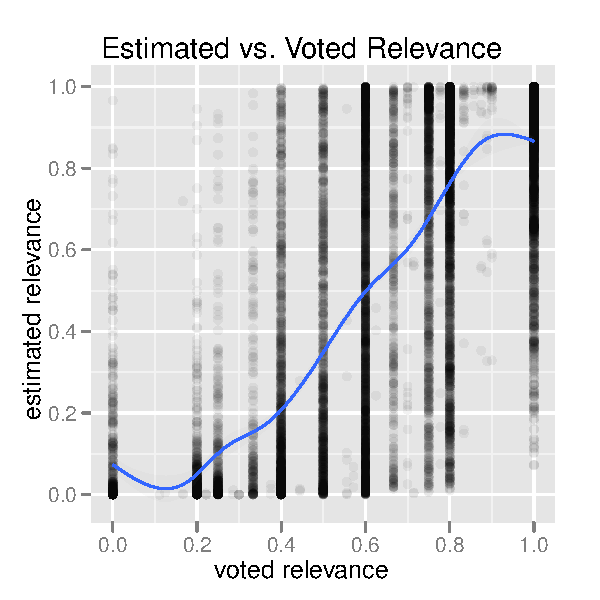
\includegraphics[height=3.0in]{img/vote_vs_estimate.pdf}
\parbox{5in}{\caption{\small {\bf Voted versus Estimated Relevance}: {\it Each point
represents a document/topic pair.  Position on the $x$ axis represents
the estimate of relevance through equally-weighted voting.  Position
on the $y$ axis represents the estimated relevance, which adjusts
votes based on estimated coder sensitivity and specificity and for the
proportion of relevant documents in the topic.  While the trend is
monotonic (other than for edge effects of the estimator), it is highly
non-linear, with estimated values being more extreme, representing
higher model-based confidence in the estimates after adjusting for
coder accuracies.}}\label{vote_vs_estimate.fig}}
\end{center}
\end{figure}
%
\begin{figure}
\begin{center}
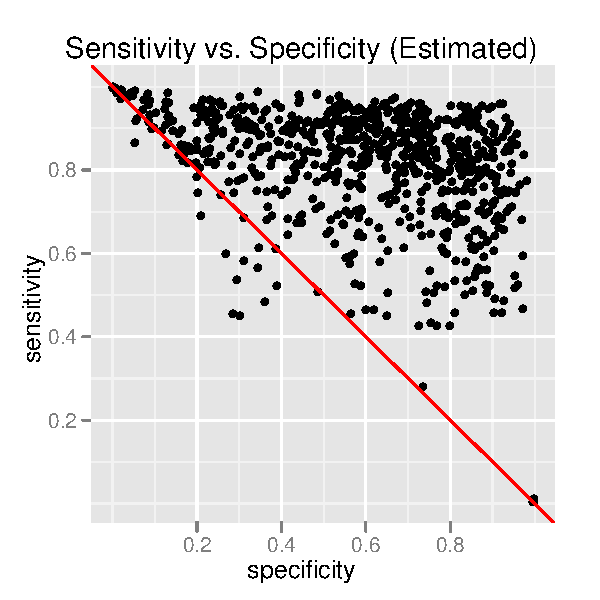
\includegraphics[height=3.0in]{img/sens_vs_spec_hat.pdf}
\parbox{5in}{\caption{\small {\bf Coder Sensivity vs.\ Specificity}: {\it Each point
represents a single coder.  The position on the $x$ axis is
specificity (i.e., accuracy on irrelevant documents, TN/[TN+FP]).  The position
on the $y$ axis is sensitivity (i.e., accuracy on relevant documents, 
TP/[TP+FN]).  The diagonal red line is chance performance, for
which sensitivity = 1 - specificity, $\theta_1[j] =
1 - \theta_0[j]$. Below the diagonal represents adversarial
performance, though the estimates shown here below the line are
likely due to sampling error rather than adversarial coding.}}%
\label{sens_spec.fig}}
\end{center}
\end{figure}
%
\begin{figure}
\begin{center}
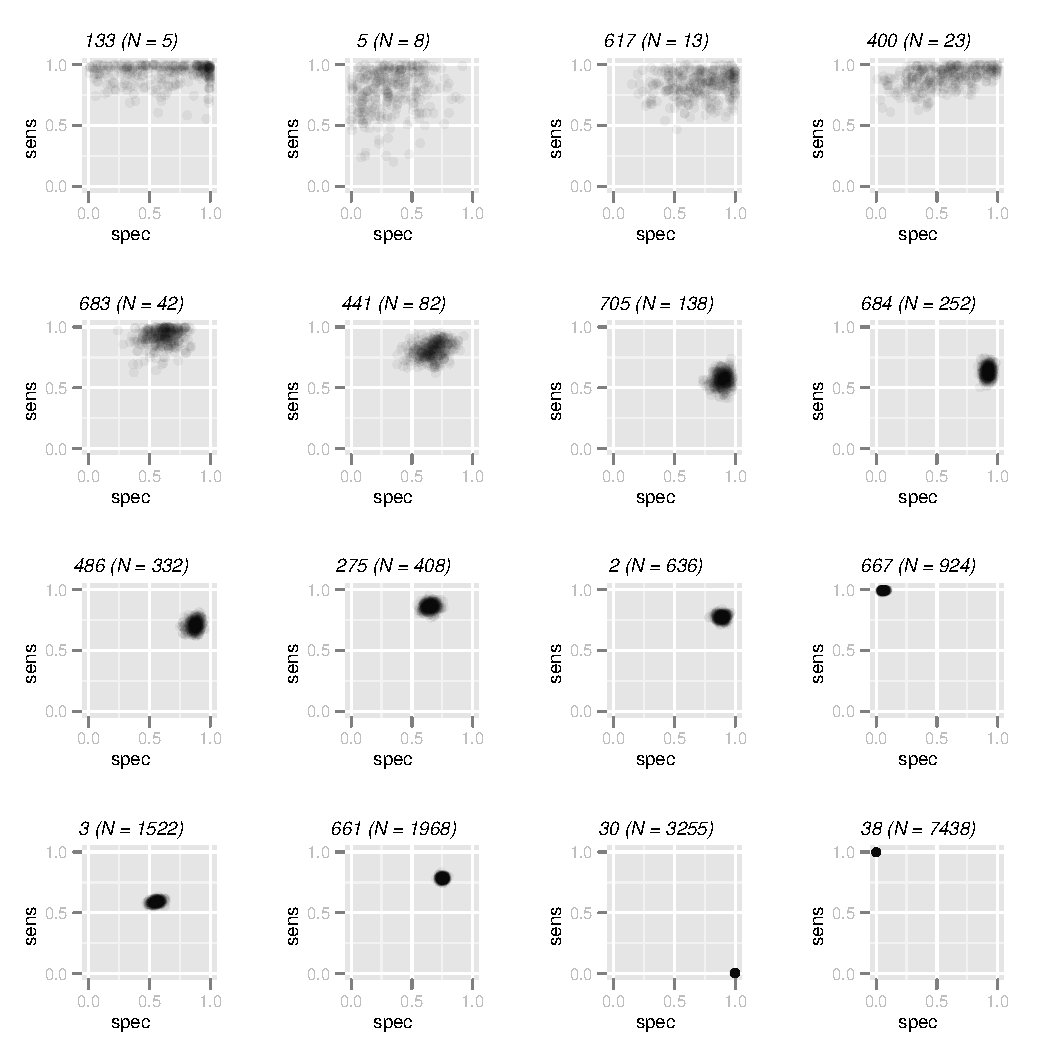
\includegraphics[height=4.0in]{img/posterior_sens_spec.pdf}
\parbox{5in}{\caption{\small {\bf Sensitivity vs.\ Specificity by Coder}: {\it  
300 Posterior samples of sensitivity and specificity from the
unsupervised model for 16  
different coders, arranged in increasing number of annotations.   
Certainty grows with the number $N$ of annotations. 
}}\label{post_sens_spec_by_anno.fig}}
\end{center}
\end{figure}
%
\begin{figure}
\begin{center}
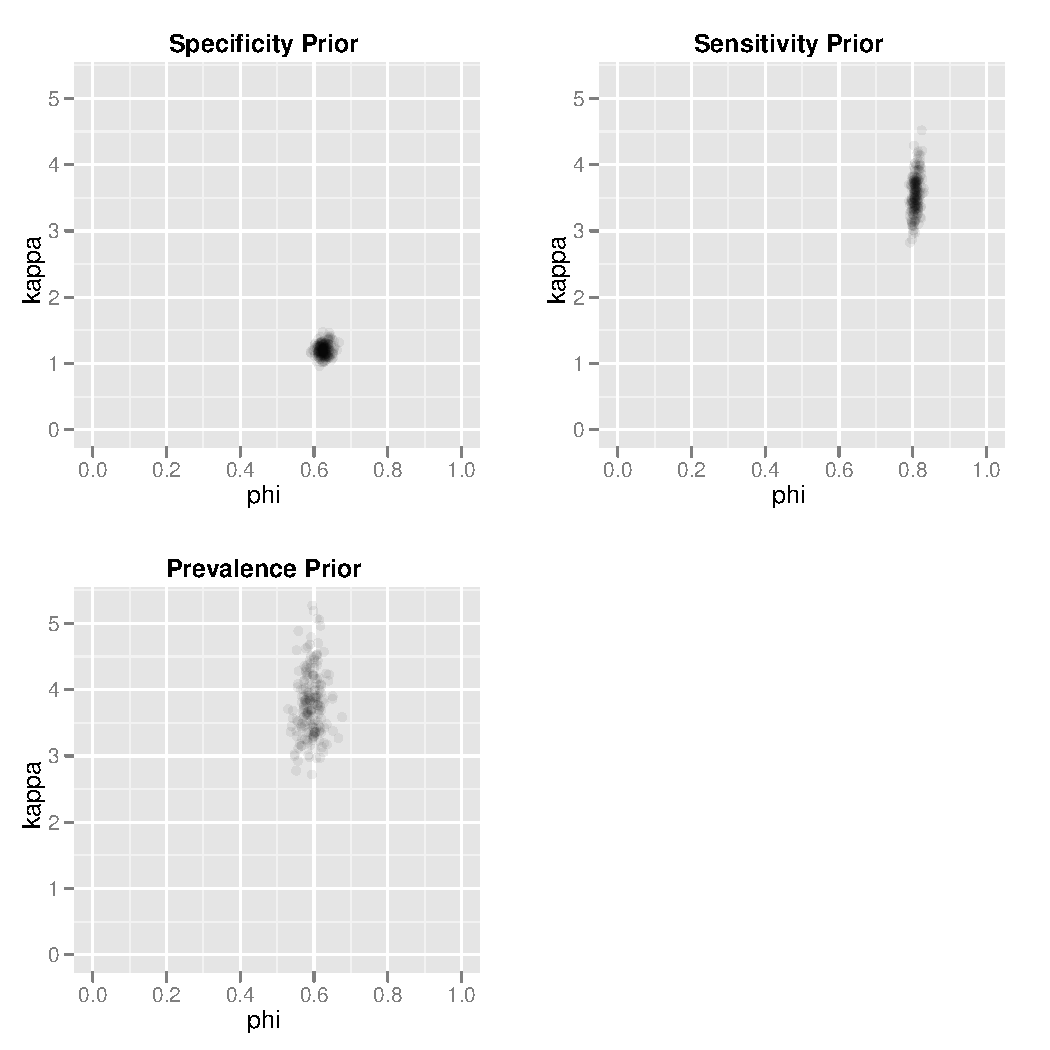
\includegraphics[height=4.0in]{img/hyperprior_post.pdf}
\parbox{5in}{\caption{\small {\bf Posteriors for Hyperpriors}: {\it  
200 Posterior samples of the hyperpriors for coder specificity
and sensitivity and prevalence of relevant documents.  The horizontal
axis is the sample for $\phi$ and the vertical for $\kappa$.  The
precision of the specificity prior is much lower than that of the
sensitivity prior and prevalence prior.  The prevalence is so high
because the corpus consists entirely of documents judged relevant
by information retrieval systems.}}}\label{hyper_post.fig}
\end{center}
\end{figure}
%


In this section, we provide several plots derived from posterior 
samples.  Figure~\ref{vote_vs_estimate.fig} shows the monotonic relationship
between voted relevance and estimated relevance in the semi-supervised
model (the ends are not extrapolated properly due to the
nearest-neighbor trend curve fitting).  

Figure~\ref{sens_spec.fig}
shows the broad range of sensitivities and specificities in evidence.
Specificity is particularly variable.  Of particular interest is the
number of coders with performance no better than chance or slightly
worse than chance (i.e., adversarial).  On pleasant feature of our
model is that it automatically discounts coders with chance
performance, as their responses are independent of the true category
and thus provide no information (see section~\ref{spam-coder-sec}).

Figure~\ref{post_sens_spec_by_anno.fig} breaks out 16 coders who
provided different number of labels.  We see that the coders with very
many labels have chance performance, with the two highest providing
all zero (irrelevant) and all one (relevant) responses respectively.  This negative correlation
between label quantity and quality is common with Amazon's Mechanical
Turk; for instance, in the data collected by Snow, O'Connor, Jurafsky
and Ng (2008), nearly half the annotations were by spam annotators
who consistently annotated large numbers of examples.


\section{Discounting Spam Coders}\label{spam-coder-sec}

A nice feature of the Dawid and Skene model is that a coder that
returns random responses will have no effect on posterior inferences
for relevance.  First not that a coder returns random responses if
their response does not depend on the category.  This happens when
sensitivity is one minus specificity, or in symbols, $\theta_{1,j} = 1
- \theta_{0,j}$.  

With such a coder, there is no effect on posteriors.  First note that
the contribution to the posterior of coder $j$ for document/topic pair
$i$ given label $y_k$ is 
%
\[
\frac{p(y_k|z_i =1)}{p(y_k|z_i = 0)}
= \frac{\theta_{j,1}}{1 - \theta_{j,0}} = 1.
\]


\section{Probabilistic Scoring}

\subsection{Log Loss Scoring}\label{log-loss-sec}

The negation of log probability is known as ``log loss'' or (sample)
cross-entropy.  It provides a natural approach to probabilistic
scoring because it is the objective function maximized on the
training data by maximum likelihood estimates and combines with the
prior for maximum a posterior (MAP) estimation.

Suppose the true answers are given in the vector
$y$, with $y_n \in \{ 0, 1 \}$ and the system repsonses are continuous
values $\hat{y}_n \in [0,1]$.  Then log probability of the truth 
$y$ estimated by system responses $\hat{y}$ is
%
\[
{\mathcal L}(y,\hat{y})  = \sum_{n=1}^N \log (y_n \, ? \, \hat{y}_n : (1 - \hat{y}_n)),
\]
%
where $(y \, ? \, x : z)$ is the ternary operator that evaluates to $x$ if $y
= 1$ and $z$ if $y = 0$.  This is just the log probability assigned to
the true labels $y$ by the model estimates $\hat{y}$.

Of course, log probability scoring only makes sense for
systems whose responses are interpretable as probabilty estimates of
relevance.

\subsection{Square Error Scoring}

Another popular method for scoring is based on squared error, which is
just the second moment of the residual.  If expected error is zero,
this
is 

Squared
error is just the sum of the squared residuals, that is, the sum
of the squared differences between the true answer and system response,
%
\[
\mbox{SE} = \sum_{n=1}^N (y_n - \hat{y}_n)^2.
\]
%
It is often presented in terms of a sample mean, where mean square
error is defined by
\[
\mbox{MSE} = \frac{1}{N} \, \sum_{n=1}^N (y_n - \hat{y}_n)^2.
\]
%
To put the error back on the same scale as the data, the square root
is often used, leading to root mean square error,
\[
\mbox{RMSE} = \sqrt{\frac{1}{N} \, \sum_{n=1}^N (y_n - \hat{y}_n)^2}.
\]
%
Given our use of Bayesian estimates minimizing expected squared loss,
our approach should do well under this evaluation method.


\subsection{Confusion Matrix Scoring}\label{confusion-matrix-eval-sec}

The obvious way to extend the standard confusion matrix measures
of precision, recall/sensitivity, and specificity is to just count
fractional responses as partly one response and partly another
response.  For instance, if the system sets $\hat{y}_n = 0.72$,
we treat that as if it was 0.72 responses of 1 and 0.28 responses
of 0. 

The problem with this approach is that it double-counts mistakes.
Consider an example topic/document pair with a 0.72 probability of
being relevant.  Now consider the scoring outcomes for a system that
returns 0.72.  There's a 72\% chance the document/topic pair is
relevant, yielding 0.72 TPs and 0.28 FNs, and a 28\% chance its
irrelevant, yielding 0.28 TNs and 0.72 FPs.  So the total
expectation is for 0.5184 TPs, 0.2016 FPs, 0.2016 FNs, and 
0.0784 TNs.  

Contrast this with the scoring outcomes for a system that returns 1,
which yields a total expectation of 0.72 TPs and 0.28 FPs.

We ran a simulation in R that took uniform samples in [0,1] for
probability estimate, then compared returning the sampled value
or rounding it to the closer of 0 or 1.  We then randomly generated
the true label according to the estimate.  Expected precision and recall were
0.75 in the quantized case and 0.66 in the probabilistic return case.

Even so, we're going to submit unquantized results and hope the
scoring is reasonable or that the organizers also provide scores for
quantized labels.  


\section{Previous Work}

Models very much like ours were applied by Dawid and Skene
(1979) to the problem of pooling the clinical diagnoses of doctors
and medical tests.  Our model generalizes Dawid and Skene's model as
well as their inference procedure.   Other than the hierarchical model
of topic relevance, these generalizations were all introduced in
(Carpenter 2008).

The first extension is to allow prevalence $\pi[t]$ to vary by topic
$t$.  Dawid and Skene only considered the case of a single topic
(though they were looking at medical diagnoses, not relevance
judgments).

The second extension is to allow an incomplete survey design.
Specifically, not all topic/document pairs need to be labeled by each
worker.  Also, a worker may label a single topic/document pair more
than once.

The third extension adds general priors for the binomial parameters
for topic prevalence of relevant documents $\pi[t]$ and worker
specificity $\theta_0[j]$ and sensitivity $\theta_1[j]$.  Dawid and
Skene did not provide a full Bayesian model, instead taking maximum
likelihood estimates (MLE), which is equivalent to maximum
a posteriori (MAP) estimation in a full model with uniform priors.

On the inference side, we provide Bayesian estimates based on 
posterior averages rather than the maximum likelihood estimates
of Dawid and Skene.  In simple hierarchical models, MLE and MAP estimates are
prone to degenerate, with likelihoods tending to infinity as 
prior variance parameters tend to zero.

Snow et al.~(2008) evaluated a fully supervised MAP estimate of Dawid
and Skene's model.  Wei and Lease (2010) evaluated MLE estimates of
the Dawid and Skene model with some supervision.  In general, any
directed graphical model may be fit using EM or Gibbs sampling with
no supervision, some supervision or full supervision; it's just a
matter of which parameters are known.   This fact has been widely
exploited in the epidemiology models where all manner of partial
supervision has been explored (particularly, positive-only follow-up
testing).

There have been several publications in the past two years that have
reinvented similar models, some with small representational twists.
The only innovation of which we are aware beyond that reported in the
epidemiology literature is that of Raykar et al.~(2010), who combined
an estimated classifier with human coders.

Also worth noting is Whitehill et al.~(2009), estimated annotation
difficulty per item in a binary task.  This approach is common
in the epidemiology literature (e.g., Uebersax and Grove 1993).
Carpenter (2008) found the posteriors for item difficulty very
uncertain given up to 10 labels per item, the problem being too many
degrees of freedom in the model.  

A trend in the epidemiology literature (e.g, Qu, Tan and Kutner 1996;
Tu, Kowalski and Jia 1999) that has so far not surfaced in the machine
learning, search and natural language processing literature as far as
we are aware is to use predictors based on the items being classified
(e.g., their source, length, language, etc.)  or the annotators (e.g.,
their training, native language, etc.).


\section{Open Source Software}

We've provided Java code for munging the basic data and R and JAGS
code for marshaling data, sampling, estimation and reporting.  The
complete set of code may be checked out of the LingPipe sandbox
using the following anonymous subversion checkout command:
% \\
% \hspace*{24pt}
% {\tt svn co https://aliasi.devguard.com/svn/sandbox/trec2011}

If that link goes away, search for the LingPipe sandbox and use
the project name {\tt trec2011}.

\section*{References}

\begin{itemize}
%
\item Carpenter, B. 2008. Multilevel Bayesian Models of
Categorical Data Annotation.  Technical Report.  LingPipe, Inc.
%
\item Dawid, A.~P.\ and A.~M.~Skene. 1979.  Maximum likelihood
estimation of observer error-rates using the EM algorithm.  {\it
Journal of the Royal Statistical Society. Series C (Applied
Statistics)} {\bf 28}(1):20--28.
%
\item Plummer, Martyn. 2010.  JAGS, version 2.2.0. 
\\ {\tt http://www-fis.iarc.fr/~martyn/software/jags/}
%
\item Karzai, Gabriella and Matthew Lease. 2011.  TREC 2011
Crowdsourcing Track.
%
\item
Qu, Yinsheng, Ming Tan, and Michael H. Kutner. 1996. Random effects
models in latent class analysis for evaluating accuracy of di-
agnostic tests. {\it Biometrics} {\bf 52}(3):797–-810.
%
\item
Raykar, Vikas C., Shipeng Yu, Linda H. Zhao, Gerardo Hermosillo
Valadez, Charles Florin, Luca Bogoni, 
and Linda Moy.  2010. Learning from crowds. {\it JMLR} {\bf 11}.
%
\item Snow, Rion, Brendan O'Connor, Daniel Jurafsky and Andrew
Y.~Ng. 2008. 
Cheap and Fast --- But is it Good? Evaluating Non-Expert Annotations
for Natural Language Tasks. 
{\it EMNLP}.
%
\item 
Tu, Xin M., Jeanne Kowalski, and Gang Jia. 1999.
Bayesian analysis of prevalence with covariates using simulation-based
techniques: applications to HIV screening. 
{\it Statistics in Medicine} {\bf 18}(22):3059– 3073.
%
\item Wei, Tang and Matthew Lease. 2011.  Semi-supervised consensus
labeling for crowdsourcing. In {\it ACM SIGIR Workshop on Crowdsourcing for
Information Retrieval}.
%
\item Whitehill, Jacob, Paul Ruvolo, Tingfan Wu, Jacob Bergsma, and
Javier Movellan. 2009. Optimal integration of labels from labelers of
unknown expertise. {\it NIPS} Poster. 
%
\end{itemize}


\end{document}


